\chapter{Parsing LL(1)}
\section{Introduzione}
Il parsing, o analisi sintattica, è una fase di compilazione  che viene utilizzata per definire la sintassi di un linguaggio di programmazione. In altre parole definisce la forma di un programma corretto. Utilizza i token \cite{libro: compilatori}, ossia sequenze di caratteri dotate di significato restituite da un analizzatore lessicale (Lexer); per produrre una rappresentazione intermedia ad albero che rappresenta la struttura grammaticale dei token. Una tipica rappresentazione è l'\textit{albero sintattico}, o \textit{syntax tree} in cui un nodo interno rappresenta un'operazione mentre i figli rappresentano gli argomenti dell'operazione; infine, questo albero prodotto, viene passato alle restanti fasi del processo di compilazione. Chiaramente, ci si aspetta che il parser sia in grado segnalare gli errori delle forme sintattiche sbagliate. In figura \ref{figParser} viene mostrato il funzionamento del parser.
\par
\vspace{0.5mm}
\begin{figure}[hbpb]\label{figParser}
	{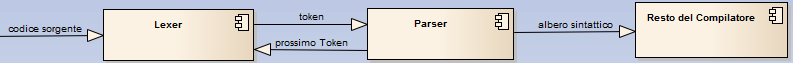
\includegraphics[height=40pt,width=420pt,scale=0.1]{parser.png}}
	\caption{\textit{Posizione del parser all'interno del compilatore.}}
\end{figure}
I metodi di parsing più comunemente utilizzate dai compilatori sono:
\begin{itemize}
	\item \textbf{Parsing top down: }la costruzione dell'albero sintattico avviene partendo dalla radice dell'albero fino ad arrivare alle foglie dell'albero;
	\item \textbf{Parsing bottom up: }la costruzione dell'albero sintattico avviene partendo dalle foglie dell'albero fino ad arrivare alla sua radice.
\end{itemize}
In questa tesi tratteremo il parsing top down in quanto il GLL parsing usa questa metodologia
\section{Grammatiche context-free}
In questo paragrafo introduciamo una notazione - \textit{la grammatica context-free} - utilizzata per specificare la sintassi dei linguaggi di programmazione. Le grammatiche sono usate per descrivere i costrutti dei linguaggi di programmazione. Ad esempio in C, il while può avere la seguente forma:
\lstset{language=C}
\begin{lstlisting}
	while (espressione) statement 
\end{lstlisting}
Questa notazione indica che il costrutto è composto dalla parola chiave \textbf{while}, una parentesi tonda aperta, un'espressione, una parentesi tonda chiusa e uno statement. Usando la variabile \textit{expr} che indica una generica espressione e la variabile \textit{stmt} per indicare lo statement, la regola di questo costrutto può essere definita nel seguente modo:
\begin{equation}\label{regolaWhile}
	stmt \to \textbf{while } ( exp ) stmt 
\end{equation}
in cui la freccia può essere letta come "può avere la forma". Questa regola prende il nome di \textbf{produzione. }All'interno della produzione la parola while, la parentesi aperta e tonda prendono il nome di \textbf{terminali}, mentre le variabili expr e stmt prendono il nome di \textbf{non terminali}.
\subsection{Definizione di grammatica}
Una grammatica context-free è una quadrupla i cui elementi sono \cite{libro: compilatori}:
\begin{enumerate}
	\item \textbf{Terminali. }I terminali sono simboli di base con cui la grammatica definisce il linguaggio. Il termine "\textit{token}" è un sinonimo di terminale.
	\item \textbf{Non-Terminali. }I non-terminali sono variabili sintattiche che denotano un insieme di stringhe. Nella produzione \ref{regolaWhile} \textit{stmt} e \textit{expr} sono non-terminali. Gli insiemi di stringhe rappresentati dai non-terminali concorrono a definire il linguaggio generato dalla grammatica.
	\item \textbf{Simbolo Iniziale. }In una grammatica uno dei non-terminali costituisce il simbolo iniziale e l'insieme di stringhe che esso denota coincide con l'intero linguaggio generato dalla grammatica. 
	\item \textbf{Produzione. }Le produzioni di una grammatica definiscono come i terminali e i non-terminali possono essere combinate a formare stringhe. Ogni produzione è formata da:
	\begin{enumerate}[(a)]
		\item un non-terminale chiamato \textbf{testa}; la produzione definisce alcune delle stringhe denotate alla sua testa;
		\item il simbolo $\to$; a volte il simbolo $\Coloneqq$ è utilizzato al posto della freccia;
		\item un \textbf{ corpo } o \textbf{lato destro} costituito da zero o più non-terminali o terminali; i componenti descrivono un modo in cui le stringhe denotate dal non-terminale della testa possono essere costruite.
	\end{enumerate}
\end{enumerate}
\subsection{Convenzioni notazionali}
In questo paragrafo vengono definite le convenzioni notazionali delle grammatiche che verranno usate nel resto della tesi.
\begin{enumerate}
	\item I seguenti simboli rappresentano i terminali:
	\begin{enumerate}[(a)]
		\item le singole lettere minuscole dell'alfabeto;
		\item i simboli degli operatori matematici e di punteggiatura;
		\item le stringhe minuscole in grassetto;
		\item le cifre numeriche.
	\end{enumerate}
	\item I seguenti simboli sono non-terminali:
	\begin{enumerate}[(a)]
		\item le singole lettere maiuscole dell'alfabeto;  
		\item se usate per descrivere i singoli costrutti della programmazione, le lettere maiuscole possono indicare i non-terminali del linguaggio.
	\end{enumerate}
	\item La testa della prima produzione è il simbolo iniziale.
	\item Un insieme di produzioni del tipo \textit{A$\to$$\alpha_{1}$}, \textit{A$\to$$\alpha_{2}$}, \dots, \textit{A$\to$$\alpha_{k}$}, con una testa comune \textit{A} (che chiamiamo \textit{A-produzioni}), 
	possono essere scritte nel seguente modo: \textit{A}$\to$$\alpha_{1}$ 
	$\mid$ $\alpha_{1}$ $\mid$ $\alpha_{2}$ \dots $\alpha_{k}$. Chiamiamo $\alpha_{1}$, $\alpha_{2}$, \dots , $\alpha_{k}$ le \textit{alternative per A}.
\end{enumerate} 
\subsection{Derivazioni}
Un albero di parsing \cite{libro: compilatori} può essere costruito mediante varie fasi di derivazioni dove, partendo dal simbolo iniziale, ad ogni passo di riscrittura un simbolo non-terminale viene sostituito con il corpo della sua produzione. Tale visione \textit{derivazionale }corrisponde al metodo di costruzione top-down degli alberi di parsing.
Facciamo un esempio. Consideriamo la seguente grammatica:
\begin{equation}\label{grammaticaEspressioni}
	E \to E + E \mid E * E \mid - E \mid ( E ) \mid \textbf{id}
\end{equation}
La produzione E $\to$ E + E significa che se E indica un'espressione alla anche E + E è un'espressione. La sostituzione di una singola E con E + E si indica con la seguente notazione:
\begin{equation}\label{derivazione1}
	E \Rightarrow E + E \Rightarrow \textbf{id} + E \Rightarrow \textbf{id} + \textbf{id}
\end{equation}
che si legge "\textit{E} deriva \textit{E + E}. La produzione \textit{E} $\to$ \textit{E + E} può essere utilizzata per sostituire qualsiasi occorrenza di \textit{E} con \textit{E + E} in una qualsiasi stringa di simboli della grammatica. La sequenza \ref{derivazione1} viene definita come una derivazione della stringa \textbf{id }+ \textbf{id} a partire da \textit{E}. Questa derivazione dimostra che la stringa \textbf{id }+ \textbf{id} è una particolare istanza di un'espressione. Ora diamo una definizione formale di concetto di derivazione. $\ll$ Consideriamo un non-terminale \textit{A} posizionata in mezzo ad una sequenza di simboli grammaticali $\alpha$\textit{A}$\beta$ dove $\alpha$ e $\beta$ sono stringhe arbitrarie di simboli grammaticali. Supponiamo che \textit{A} $\to$ $\gamma$ sia una produzione. In tal caso possiamo scrivere $\alpha$\textit{A}$\beta$ $\Rightarrow$ $\alpha$$\gamma$$\beta$, in cui il simbolo $\Rightarrow$ significa "deriva in un solo passo". Quando abbiamo una sequenza di passi di derivazione del tipo $\alpha_{1}$ $\Rightarrow$ $\alpha_{2}$ $\Rightarrow$ \dots $\Rightarrow$ $\alpha_{n}$ in cui possiamo riscrivere $\alpha_{1}$ come $\alpha_{n}$ diremo $\alpha_{1}$ \textit{deriva }$\alpha_{n}$. Per esprimere che una stringa "deriva in zero o più passi" una nuova stringa utilizziamo il simbolo $\overset{*}{\Rightarrow}$. Quindi, 
\begin{enumerate}
	\item $\alpha$ $\overset{*}{\Rightarrow}$ $\alpha$, per qualsiasi stringa $\alpha$;
	\item  se $\alpha$ $\overset{*}{\Rightarrow}$ $\beta$ e $\beta$ $\Rightarrow$ $\gamma$, allora $\alpha$ $\overset{*}{\Rightarrow}$ $\gamma$.
\end{enumerate} 
Inoltre il simbolo $\overset{+}{\Rightarrow}$ significa "deriva in uno o più passi. \par
Se \textit{S} $\overset{+}{\Rightarrow}$ $\alpha$, dove \textit{S} è il simbolo iniziale della grammatica \textit{G}, diciamo che $\alpha$ è una \textbf{forma sentenziale}  di \textit{G}. Una forma sentenziale può contenere sia terminali che non terminali e può essere vuota. Una \textbf{sentenza} o \textbf{frase} di \textit{G} è una forma sentenziale che non contiene nessun non-terminale. Il \textbf{linguaggio generato} da una grammatica \textit{G} è l'insieme di tutte le sue frasi. Quindi una stringa di terminali \textit{w} appartiene a \textit{L(G)}, il linguaggio generato da \textit{G}, se e solo se \textit{w} è una frase di \textit{G}, cioè se \textit{S} $\overset{*}{\Rightarrow}$ \textit{w}. Un linguaggio che può essere generato da una grammatica è detto un \textbf{linguaggio libero dal contesto}. Se due grammatiche generano lo stesso linguaggio sono dette \textbf{equivalenti}.$\gg$ La stringa \textbf{id}+\textbf{id} è una frase della grammatica \ref{grammaticaEspressioni} poichè esiste la derivazione \ref{derivazione1}. Le sequenze di derivazioni prevedono che ad ogni vengano fatte due scelte: la prima scelta consiste nello scegliere il non-terinale da sostituire; la seconda scelta consiste nello scegliere una delle produzioni in cui il non-terminale scelto risulta essere la testa della produzione. Infatti nella derivazione \ref{derivazione1} ogni non-terminale è sostituito con il corpo della produzione corrispondente. Ogni non-terminale da sostituire viene selezionato in questo modo:
\begin{enumerate}
	\item nelle \textit{derivazioni sinistre} si sceglie sempre il non-terminale più a sinistra. La derivazione \ref{derivazione1} è una derivazione a sinistra.
	\item  nelle \textit{derivazioni destre} si sceglie sempre il non-terminale più a destra. 
\end{enumerate}
\subsection{Alberi di parsing}
Un \textbf{albero di parsing} è \cite{libro: compilatori} una rappresentazione grafica di una derivazione che non dipende dall'ordine in cui le produzioni sono utilizzate per rimpiazzare i non-terminali. Ogni nodo interno rappresenta l'applicazione di una produzione ed è etichettato con il non-terminale che indica la testa della  produzione. I figli di questo nodo sono etichettati con i simboli che appaiono nel corpo della produzione utilizzata per sostituire il non-terminale. Un esempio di albero di parsing relativo alla stringa \textbf{id }+\textbf{ id} è mostrato nella figura 2.2.
\begin{figure}[hbpb]\label{albero}
	\centering
	\begin{forest}
		[E
		  [E
		  [\textbf{id}]
		  ]
		  [+]
		  [E
		  [\textbf{id}]
		  ]
		]
	\end{forest}
	\caption{\textit{Albero di parsing relativo alla stringa} \textbf{id} + \textbf{id} }
\end{figure}
Le foglie dell'albero di parsing sono etichettate con terminali o non-terminali che, letti da sinistra verso destra formano una forma sentenziale chiamata \textbf{frontiera} dell'albero. Ora tramite un esempio mostreremo come viene costruito un albero sintattico. \par
\begin{figure}[hbpb]\label{passiAlbero}
	\centering
	\begin{forest}
		[E
		[E]
		[+]
		[E]
		]
	\end{forest}
	$\Rightarrow$    
	\begin{forest}
		[E
		[E
		[\textbf{id}]
		]
		[+]
		[E]
		]
	\end{forest}
	$\Rightarrow$    
	\begin{forest}
		[E
		[E
		[\textbf{id}]
		]
		[+]
		[E
		[\textbf{id}]
		]
		]
	\end{forest}
	\caption{\textit{Sequenza di alberi di parsing relativi alla derivazione }\ref{derivazione1}}
\end{figure}
In figura 2.3 viene rappresentata la sequenza di alberi sintattici costruiti dalla derivazione \ref{derivazione1}. Il primo passo della derivazione \textit{E} $\Rightarrow$ \textit{E} + \textit{E} prevede di aggiungere come radice dell'albero sintattico il simbolo iniziale \textit{E} e come figli \textit{E}, +, ed \textit{E} che corrisponde al corpo della produzione \textit{E} + \textit{E}. Al secondo passo della derivazione \textit{E} $\Rightarrow$ \textbf{id} + \textit{E} aggiungiamo al nodo più a sinistra \textit{E} il nodo figlio \textbf{id}. Così facendo otteniamo al terzo passo il corrispondente albero sintattico per la stringa \textbf{id} + \textbf{id}.
\subsection{Ambiguità}
Una grammatica viene definita \textbf{ambigua} se produce più di un albero sintattico. In altre parole una grammatica ambigua presenta \cite{libro: compilatori} più di una derivazione destra o sinistra per una frase. Facciamo un esempio. Prendiamo in considerazione la grammatica \ref{grammaticaEspressioni} e la frase \textbf{id}+\textbf{id}*\textbf{id}; questa frase presenta due alberi di parsing che sono:\par
\begin{figure}[hbpb]\label{alberibis}
	\centering
	\begin{forest}
		[E
		[E[\textbf{id}]]
		[+]
		[E
		[E[\textbf{id}]] [*][E[\textbf{id}]]]
		]
	\end{forest}
	\begin{forest}
		[E
		[E [E[\textbf{id}]] [+][E[\textbf{id}]]]
		[*]
		[E[\textbf{id}]]
		]
	\end{forest}
	\caption{\textit{Alberi di parsing relativi alla stringa } \textbf{id}+\textbf{id}*\textbf{id}}
\end{figure}
Di conseguenza ciò dimostra che la grammatica \ref{grammaticaEspressioni} risulta essere ambigua.
\subsection{Ricorsione a sinistra}
Una grammatica viene definita \textbf{ricorsiva a sinistra} \cite{libro: compilatori} se ha un non-terminale \textit{A} per cui esiste una derivazione \textit{A}$\overset{+}{\Rightarrow}$ \textit{A}$\alpha$ della stringa $\alpha$. Un esempio di ricorsione a sinistra è la seguente produzione:
\[
	term \to term + fact
\]
Le grammatiche ricorsive a sinistre risultano essere problematiche da gestire da parser a discesa ricorsiva perchè entrano in un ciclo infinito. Supponiamo che la procedura per il simbolo \textit{expr} decide di applicare questa produzione. Il corpo inizia con \textit{expr} per cui la procedura per \textit{expr} viene invocata ricorsivamente. Poichè il simbolo di lookahead cambia solo quando si verifica una corrispondenza con un terminale del corpo della produzione, nulla cambia sulla stringa in ingresso che si sta analizzando. Di conseguenza la procedura \textit{expr()} viene chiamata di nuovo e così fino all'infinito.
\section{Parsing top down}
Il parsing top down è una tecnica che prevede di costruire l'albero di parsing per una determinata stringa partendo dalla radice dell'albero fino ad arrivare alle foglie che rappresentano i simmboli della stringa. Questo parsing effettua derivazioni a sinistra sulle stringhe che analizza. Infatti ad ogni passo di computazione il parsing top down cerca di trovare un possibile corpo di produzione da sostituire ad ogni non-terminale. Una volta fatto ciò cerca di trovare una corrispondenza tra i simboli della stringa in ingresso e tra i simboli del corpo della produzione. In questo paragrafo analizzeremo i principi e gli strumenti che usa il parsing top down. Verrà presentato il parsing a discesa ricorsiva che richiede \textit{backtracking} per trovare la produzione opportuna da applicare al non-terminale. Successivamente introdurremo le funzioni FIRST e FOLLOW utilizzate per scegliere la produzione da applicare in base al simbolo in input che si sta analizzando. Poi parleremo delle grammatiche LL(1) ed infine dei parser predittivi che usano le funzioni FIRST e FOLLOW per scegliere le produzioni da sostituire.
\subsection{Parsing a discesa ricorsiva}
ioo
\subsection{Funzioni FIRST e FOLLOW}
eicuei
\subsection{Gramatiche LL(1)}
ceiocmeo
\subsection{Parsing predittivo non ricorsivo}
klmlm
\section{Conclusioni}
nknnin